\documentclass[]{article}
\usepackage{lmodern}
\usepackage{amssymb,amsmath}
\usepackage{ifxetex,ifluatex}
\usepackage{fixltx2e} % provides \textsubscript
\ifnum 0\ifxetex 1\fi\ifluatex 1\fi=0 % if pdftex
  \usepackage[T1]{fontenc}
  \usepackage[utf8]{inputenc}
\else % if luatex or xelatex
  \ifxetex
    \usepackage{mathspec}
  \else
    \usepackage{fontspec}
  \fi
  \defaultfontfeatures{Ligatures=TeX,Scale=MatchLowercase}
\fi
% use upquote if available, for straight quotes in verbatim environments
\IfFileExists{upquote.sty}{\usepackage{upquote}}{}
% use microtype if available
\IfFileExists{microtype.sty}{%
\usepackage{microtype}
\UseMicrotypeSet[protrusion]{basicmath} % disable protrusion for tt fonts
}{}
\usepackage[unicode=true]{hyperref}
\hypersetup{
            pdfborder={0 0 0},
            breaklinks=true}
\urlstyle{same}  % don't use monospace font for urls
\usepackage{graphicx,grffile}
\makeatletter
\def\maxwidth{\ifdim\Gin@nat@width>\linewidth\linewidth\else\Gin@nat@width\fi}
\def\maxheight{\ifdim\Gin@nat@height>\textheight\textheight\else\Gin@nat@height\fi}
\makeatother
% Scale images if necessary, so that they will not overflow the page
% margins by default, and it is still possible to overwrite the defaults
% using explicit options in \includegraphics[width, height, ...]{}
\setkeys{Gin}{width=\maxwidth,height=\maxheight,keepaspectratio}
\IfFileExists{parskip.sty}{%
\usepackage{parskip}
}{% else
\setlength{\parindent}{0pt}
\setlength{\parskip}{6pt plus 2pt minus 1pt}
}
\setlength{\emergencystretch}{3em}  % prevent overfull lines
\providecommand{\tightlist}{%
  \setlength{\itemsep}{0pt}\setlength{\parskip}{0pt}}
\setcounter{secnumdepth}{0}
% Redefines (sub)paragraphs to behave more like sections
\ifx\paragraph\undefined\else
\let\oldparagraph\paragraph
\renewcommand{\paragraph}[1]{\oldparagraph{#1}\mbox{}}
\fi
\ifx\subparagraph\undefined\else
\let\oldsubparagraph\subparagraph
\renewcommand{\subparagraph}[1]{\oldsubparagraph{#1}\mbox{}}
\fi

% set default figure placement to htbp
\makeatletter
\def\fps@figure{htbp}
\makeatother


\date{}

\begin{document}

\emph{La patologia del ginocchio (Vaienti)}

\emph{Anatomia}

Il ginocchio è una articolazione in cui si incontrano tre ossa: femore,
tibia e rotula. La rotula è un osso sesamoide, incastonata dentro un
unico tendine che parte dal quadricipite e termina sulla tuberosità
tibiale; si parla di tendine del quadricipite e tendine rotuleo quanto
in realtà è un apparato estensorio unico.

La rotula serve a migliorare il braccio di leva. Esiste poi la
cosiddetta ``pes anserinus'' o zampa d'oca formata dalla convergenza dei
tendini di semitendinoso, gracile e sartorio. Il tratto ileo-tibiale
termina sul tubercolo del Gerdy (può dare tendiniti, fasciti). A livello
della zampa d'oca, del tratto ileo-tibiale, del bicipite femorale, vi
sono le borse che possono infiammarsi (borsiti).

Dal punto di vista biomeccanico, l'articolazione del ginocchio è una
\textbf{doppia articolazione condiloidea}

Tra i 2 condili femorali e i 2 emipiatti tibiali, con in più
l'articolazione trocleare tra la troclea femorale e la faccia profonda
della rotula.

È un'articolazione che non è dotata di una grossa stabilità intrinseca,
anche perché le superfici articolari non sono tanto coese tra loro, nel
senso che la complessità dei condili femorali non è controbilanciata
dalla stabilità dei due legamenti.

\emph{Ci sono, quindi, delle strutture che aumentano la stabilità di
questa articolazione dando una stabilità attiva e una passiva.}

\emph{Gli \textbf{stabilizzatori passivi} sono rappresentati dai
menischi e dalle strutture capsulo-legamentose.}

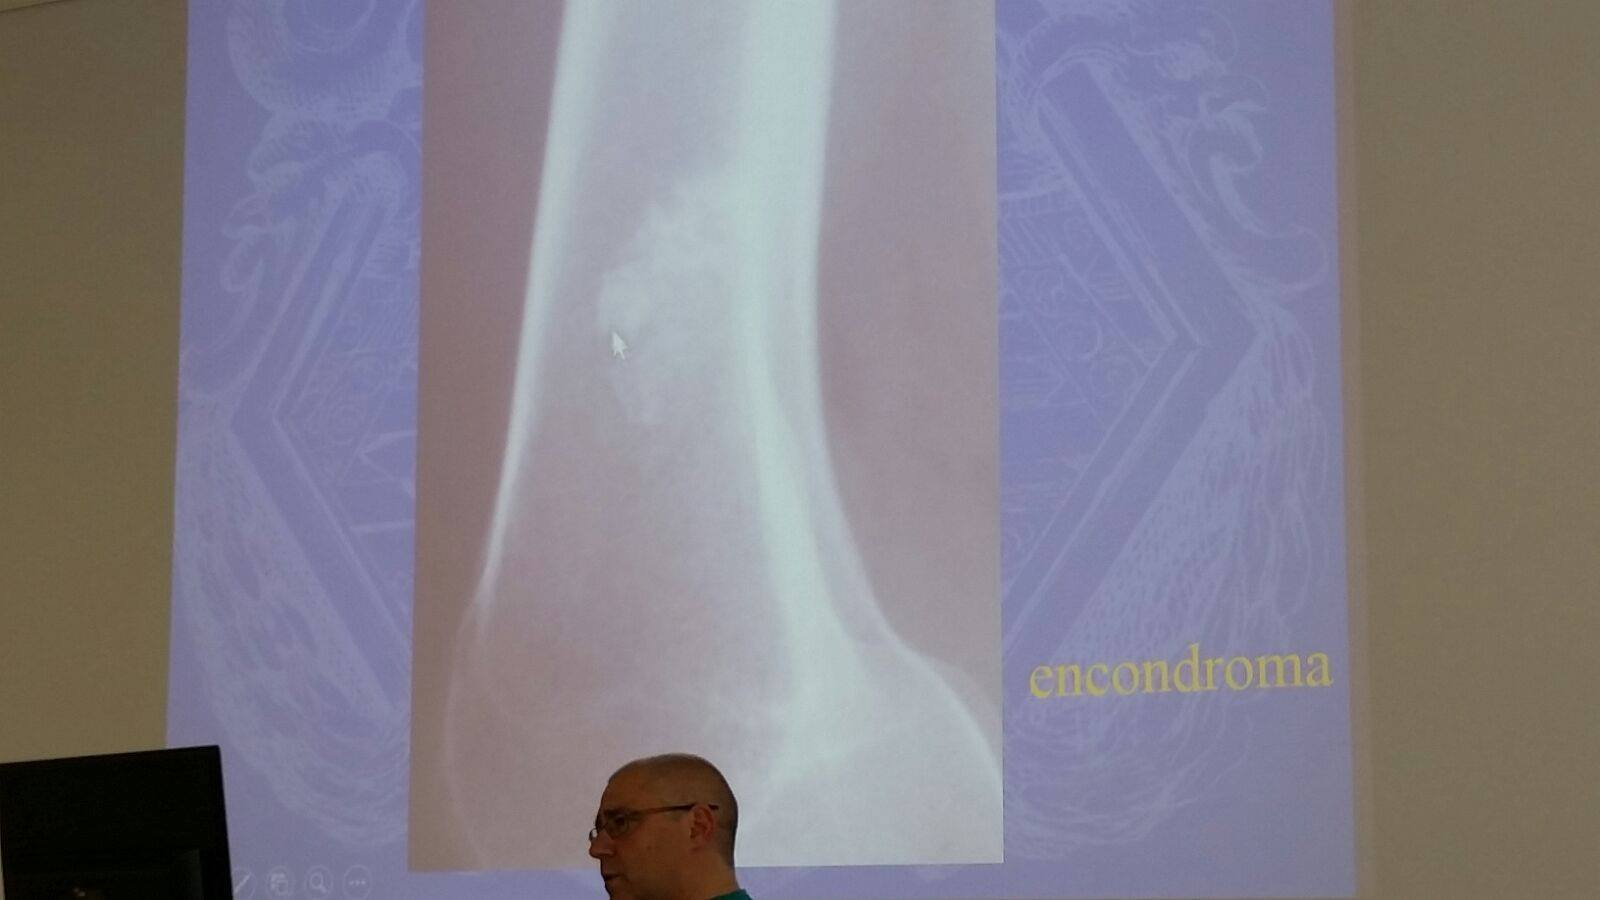
\includegraphics[width=3.47847in,height=2.96806in]{media/image1.jpeg}

\begin{itemize}
\item
  \emph{\textbf{Menischi}: sono due fibrocartilagini di struttura
  triangolare, uno mediale e uno laterale e hanno la funzione sia di
  aumentare la congruenza articolare (aumentare la concavità dei piatti
  tibiali), sia di essere dei veri e propri ammortizzatori articolari. }
\end{itemize}

\begin{quote}
\emph{Il menisco mediale è più fisso rispetto al menisco laterale, nel
senso che si muove meno nei movimenti di flesso-estensione del
ginocchio, ed anche per questa sua caratteristica, è più soggetto} alle
lesioni nei traumi distorsivi del ginocchio.
\end{quote}

\begin{itemize}
\item
  \emph{\textbf{Legamenti crociati} anteriore (LCA) e posteriore (LCP)
  sono importanti stabilizzatori del ginocchio sia in senso
  antero-posteriore che in senso rotazionale.}
\item
  \emph{\textbf{Legamenti collaterali} mediale (LCM) e laterale (LCL)
  sono importanti stabilizzatori medio-laterali del ginocchio ed anche
  stabilizzatori rotazionali.}
\end{itemize}

\emph{Gli \textbf{stabilizzatori attivi} del ginocchio sono costituiti
dalle \textbf{strutture muscolari} che decorrono attorno
all'articolazione del ginocchio:}

\begin{itemize}
\item
  \emph{anteriormente il muscolo quadricipite con il tendine
  quadricipitale,}
\item
  \emph{muscoli posteriori rappresentati dai muscoli della zampa d'oca,
  dai flessori del ginocchio ed anche dal muscolo gastrocnemio.}
\end{itemize}

La rotula scivola nella troclea femorale. Le faccette delle rotula sono
poggiate sulla superficie dei condili; se c'è un disassamento
dell'apparato estensore questo rapporto tra concavità e convessità si
perde e si possono creare delle iperpressioni e delle sofferenze
cartilaginee. La borsa prerotulea e quella infrarotulea (in rapporto con
il tendine rotuleo), inoltre, possono andare incontro a borsiti quando
si sta troppo tempo inginocchiati o in seguito ad un trauma. La rotula
poggia su un cuscinetto adiposo, il \emph{pannicolo di Hoffa}, che si
può infiammare.

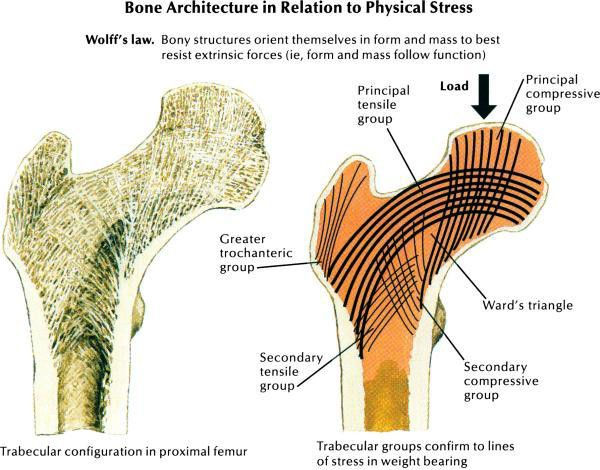
\includegraphics[width=6.45833in,height=6.28125in]{media/image2.jpeg}

\emph{Versamenti Articolari}

Nella capsula sinoviale si raccoglie un liquido che può essere un
essudato, sangue oppure pus; il versamento si raccoglie in questa cavità
virtuale che può distendersi.

Quando si supera la capacità recettiva della cavità, si possono aprire
delle piccole asole a livello della membrana cribrosa e da queste può
uscire del liquido con la formazione delle \textbf{cisti poplitee di
Baker} (questa cisti non si può formare anteriormente perché c'è la
rotula, ma trova sbocco nel cavo popliteo posteriormente). Alla base
della cisti di Baker c'è il versamento articolare (non esiste la
malattia ``cisti di Baker'').

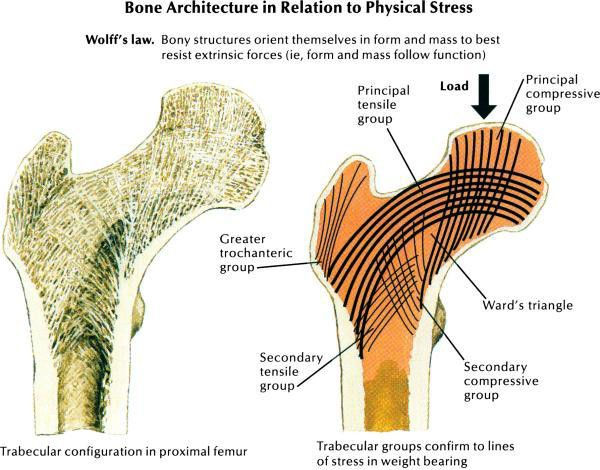
\includegraphics[width=3.42708in,height=2.64583in]{media/image3.jpeg}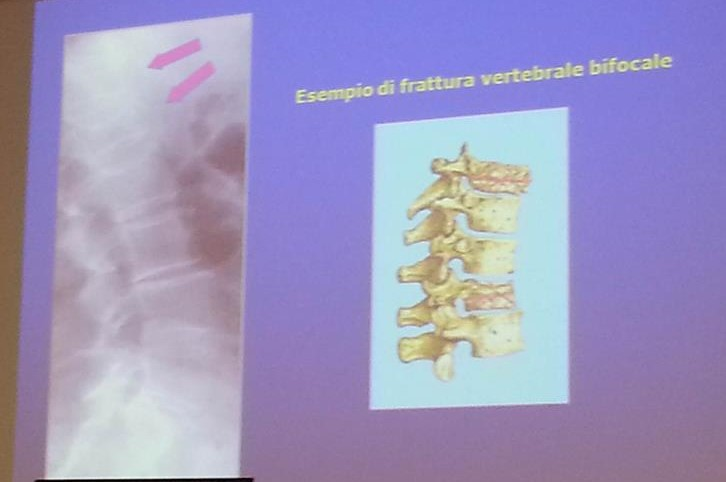
\includegraphics[width=2.91667in,height=2.63542in]{media/image4.jpeg}

Fanno parte dell'articolazione i condili, la troclea femorale, i
legamenti crociati anteriore e posteriore, i menischi, i legamenti
collaterali.

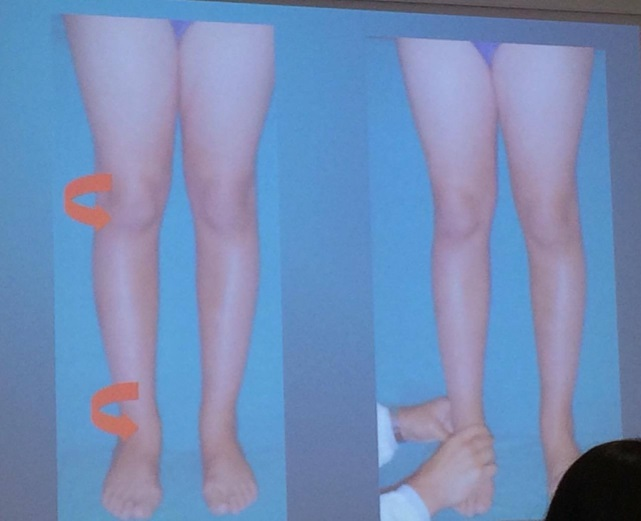
\includegraphics[width=3.01250in,height=2.04375in]{media/image5.jpeg}I
\textbf{crociati} sono \textbf{intraarticolari ma extrasinoviali}: sono
rivestiti da una guaina che isola questi legamenti dall'ambiente umido
sinoviale → l'equazione: rottura del legamento crociato = emartro non va
fatta perché ci può essere una rottura del crociato ``in continuità''
che non interrompe la sua guaina e non dà versamento ematico),

Il pivot centrale è fatto dal crociato posteriore e dal crociato
anteriore che si inseriscono rispettivamente verso l'interno e verso
l'esterno della gola. Esistono 2 menischi: esterno e interno. Il menisco
esterno è più chiuso, infatti esiste una patologia chiamata menisco
discoide (anziché essere aperto come una ``c'' è chiuso come una ``o'';
tipico di femmine adolescenti che sentono un forte schiocco in quella
sede.

Varismo e Valgismo

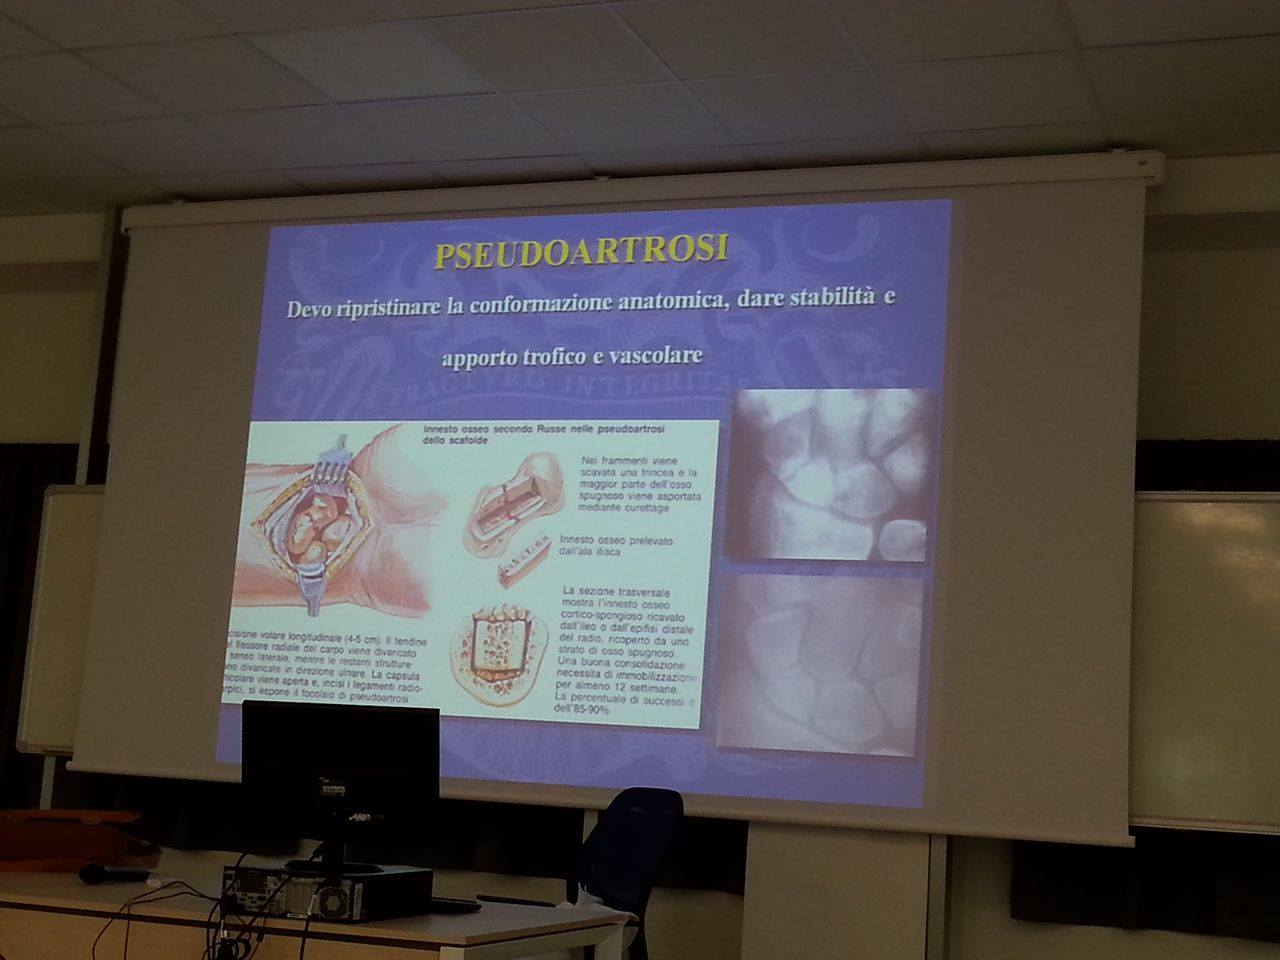
\includegraphics[width=3.13611in,height=2.16944in]{media/image6.jpeg}\emph{L'arto
inferiore normale ha una conformazione normale che si esplica a livello
del ginocchio con la presenza di un angolo di valgismo fisiologico. }

\emph{Si parla di deviazione assiale patologica, quando si esce dai
range di normalità: in tal caso si può avere valgismo o varismo:}

\begin{itemize}
\item
  \emph{Il ginocchio \textbf{varo} è il tipico "ginocchio a parentesi"
  del calciatore; }
\item
  \emph{il ginocchio \textbf{valgo} è il tipico "ginocchio a X" spesso
  presente nei soggetti che hanno i piedi piatti che hanno
  tendenzialmente un aumento del valgismo normale. }
\item
  \emph{Il ginocchio è normale quando presenta alcuni gradi di valgismo
  fisiologico: circa 7°. }
\end{itemize}

\begin{quote}
\emph{Nell'arto inferiore bisogna tenere in considerazione due assi
importanti: \textbf{l'asse anatomico}, che nasce dall'unione, a livello
del ginocchio, tra una retta che passa perfettamente al centro della
diafisi del femore che si unisce con una retta che passa perfettamente
al centro della diafisi della tibia. L'intersezione di queste rette
definisce un angolo di valgismo fisiologico aperto verso l'esterno di
173°-177°.}

\emph{\textbf{L'asse meccanico} è una retta tesa tra il centro della
testa del femore e il centro della caviglia che passa perfettamente al
centro del ginocchio. In questa condizione di normalità, tutte le forze
di carico vengono distribuite uniformemente su tutto il piatto tibiale.
}

\emph{• Nel ginocchio varo, invece, questa condizione è sovvertita:
l'angolo di valgismo fisiologico è maggiore rispetto al range di
normalità, l'asse anatomico è tutto spostato verso l'interno del
ginocchio e questo comporta una concentrazione dei carichi prevalenti
sulla parte mediale dell‟articolazione. }

\emph{• Nel ginocchio valgo si riscontra la situazione opposta: l'angolo
di valgismo fisiologico è minore rispetto al range di normalità, e
l'asse meccanico è tutto spostato lateralmente, perciò tutte le forze di
carico sono concentrate maggiormente sulla parte laterale
dell‟articolazione.}
\end{quote}

La patologia può essere :

\begin{itemize}
\item
  Degenerativa
\item
  Infiammatoria
\item
  Traumatica
\item
  Neoplastica
\end{itemize}

PATOLOGIA TRAUMATICA

\begin{itemize}
\item
  \textbf{Fratture }
\item
  \textbf{Distorsioni }
\item
  \textbf{Lussazioni }
\end{itemize}

\emph{Distacchi Epifisari}

Sono le fratture tipiche dei bambini. Si distacca l'epifisi perché la
cartilagine di accrescimento non si è ancora saldata (ossificata),
esiste quindi un locus minoris resistentiae che può dare origine a
questa dissociazione. Il distacco epifisario può essere:

\begin{itemize}
\item
  \textbf{Puro }
\item
  \textbf{Misto} (coinvolge l'epifisi, la cartilagine di accrescimento e
  anche parte dell'osso)
\item
  \textbf{Completo }
\item
  \textbf{Transepifisario}
\end{itemize}

Il chirurgo interviene bloccando l'epifisi, la metafisi e la frattura
transepifisaria con delle graffette che poi vengono rimosse per
permettere il corretto accrescimento dell'osso. Le fratture gravi e
importanti vanno ridotte nel minor tempo possibile perché altrimenti
possono alterare l'accrescimento

A seconda del danno che subiscono le cellule ci può essere un
accrescimento in eccesso o in difetto: le cellule possono avere un danno
talmente grave e quindi \emph{non proliferare più}, in questo caso
l'epifisi cresce soltanto nella porzione non colpita.

In seguito al danno le cellule coinvolte possono \emph{proliferare di
più} e ci può essere una crescita monolaterale dell'epifisi. I difetti
che ne possono derivare sono \textbf{valgismo o varismo}; i distacchi
epifisari vanno sempre guardati con molta severità.

Le fratture del ginocchio

\begin{itemize}
\item
  \textbf{Extra-articolari} (interessano la metafisi ma non l'epifisi)
  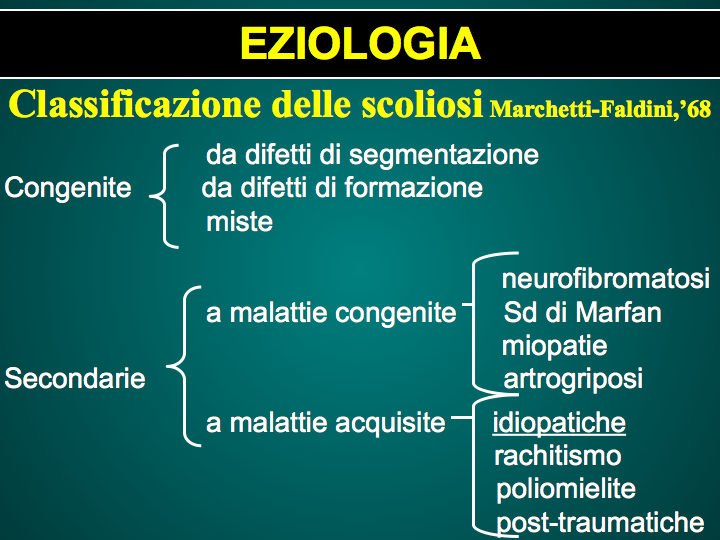
\includegraphics[width=3.56250in,height=2.58333in]{media/image7.png}
\item
  \textbf{Articolari} (la frattura si spinge dentro l'articolazione ) →
  esempio: radiografia di frattura a ``y'' metafiso-epifisaria
\end{itemize}

\begin{quote}
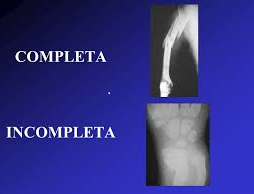
\includegraphics[width=3.04167in,height=2.45833in]{media/image8.png}
\end{quote}

Tutte le \textbf{fratture articolari} comportano un danno cartilagineo e
spesso legamentoso.

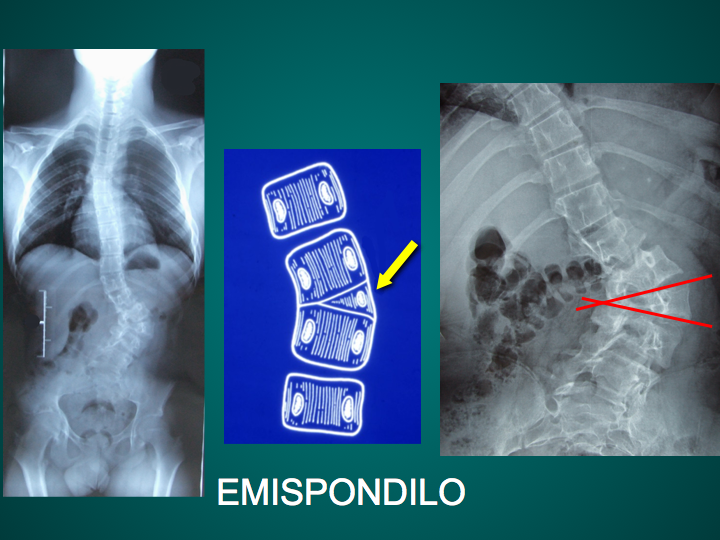
\includegraphics[width=3.35417in,height=2.08681in]{media/image9.png}Un
quadro particolarmente grave è quello del ``\emph{floating knee}'': il
ginocchio fluttua a causa di una frattura femorale (a monte) e una
tibiale (a valle) che rendono totalmente instabile il ginocchio. Si
presenta solitamente in pazienti con politraumi o comunque instabili; si
verifica la morte nel 5-15\% di questi pazienti per il quadro globale
critico (pz politraumatico: danni neurologici, vascolari, legamentosi)

Frattura a sconquasso epifisario con frattura transrotulea → immagine

NB: la cartilagine è un tessuto che non replica, non cicatrizza, al
massimo può fare dei ponti fibrosi ma la cartilagine ialina non si forma
più. In una frattura esposta alcuni pezzi d'osso che vengono persi e
altri che vengono schiacciati e compenetrati lasciano un vuoto che viene
colmato dal chirurgo con dei sostituti ossei.

\emph{Fratture del piatto tibiale}

Classificazione di Schatzker

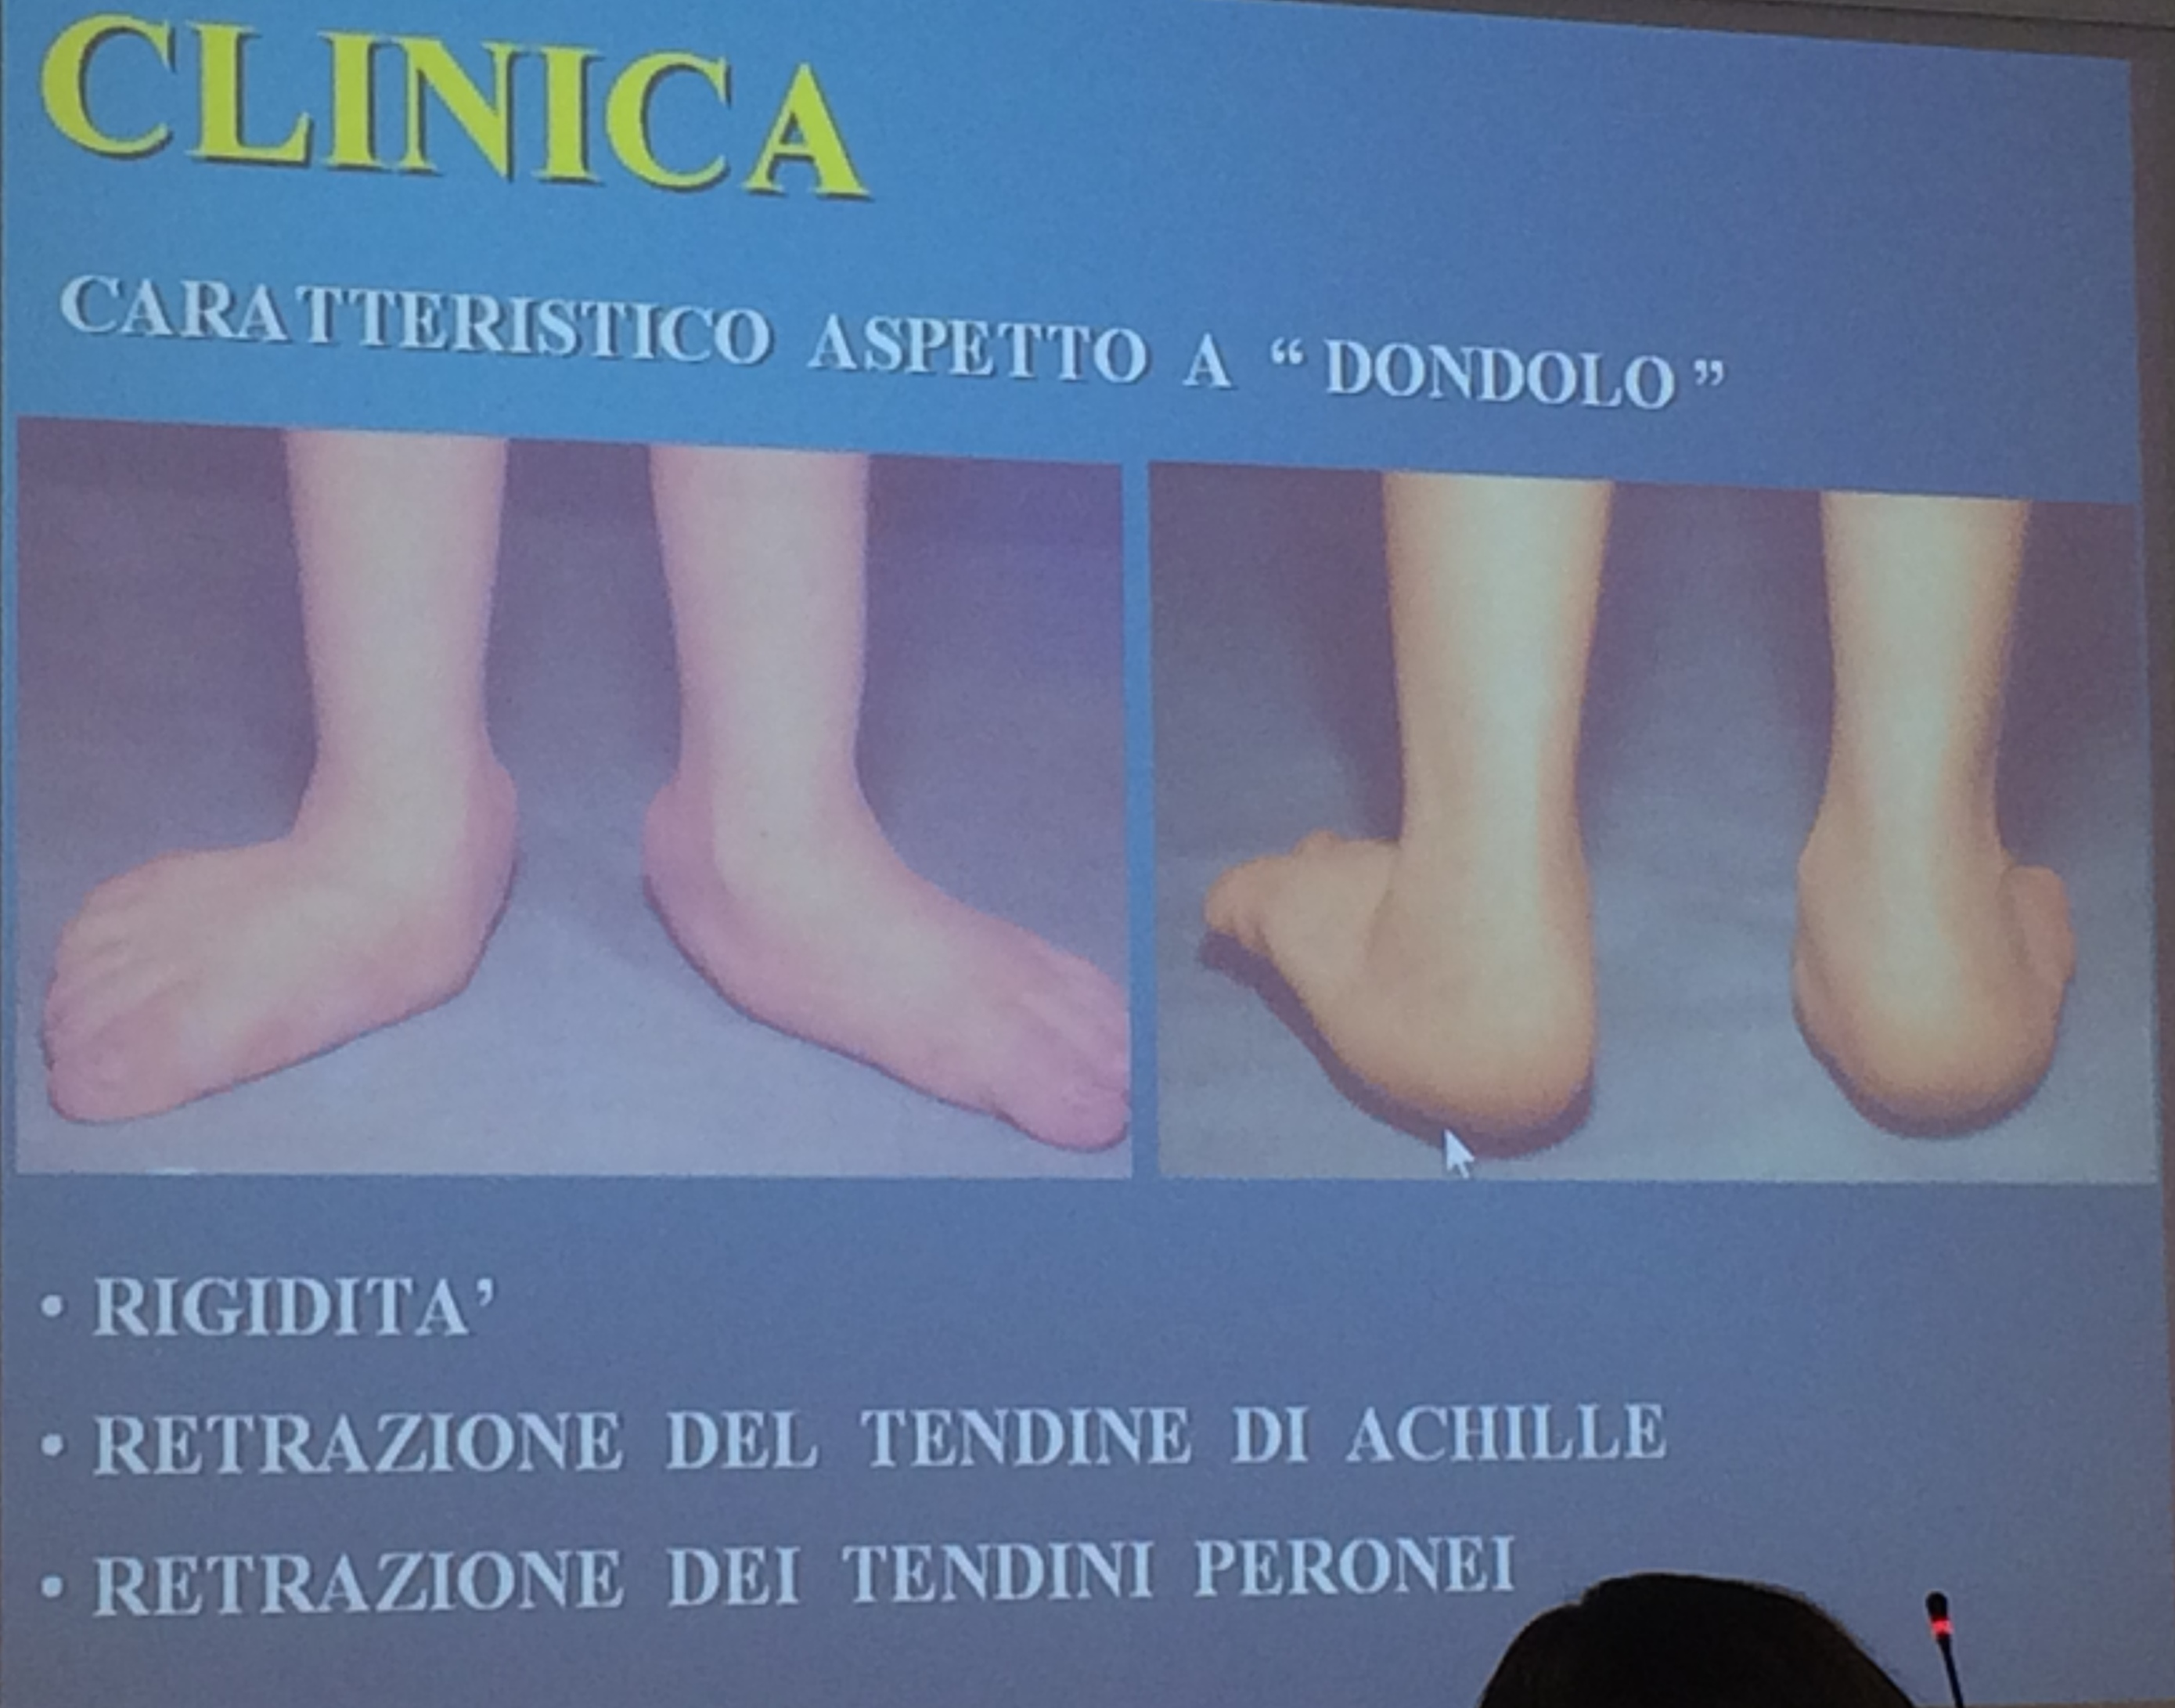
\includegraphics[width=6.68750in,height=1.77083in]{media/image10.jpeg}

Tipo 1→ frattura semplice

Tipo 2→ il frammento intermedio è affondato

Tipo 3→ c'è un crollo più o meno ampio

Tipo 4→ rottura a y

Tipo 5→ rottura dei 2 condili

Tipo 6→ la frattura si estende verso il basso

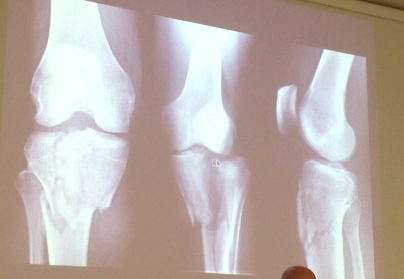
\includegraphics[width=3.65625in,height=2.53125in]{media/image11.png}

\emph{Caso di frattura al piatto tibiale}: caso di un ragazzo caduto
mentre sciava. Tutto il peso è finito in modo violento sul ginocchio →
il condilo si è incuneato dentro il piatto tibiale. Coinvolgimento e
alterazione di menisco, crociati, cartilagine. Per poter sistemare il
piatto tibiale il chirurgo è intervenuto sollevando il menisco e
applicando una o 2 placche contrapposte.

NB: le fratture articolari aprono sempre la strada a un disagio
immediato oppure a un disagio futuro e cioè ad una artrosi
post-traumatica .

DISTORSIONI

\emph{È l'insieme delle lesioni capsulo-legamentose prodotte da una
sollecitazione traumatica che tende a modificare temporaneamente i
reciproci rapporti dei capi articolari}.

\begin{itemize}
\item
  \emph{Una \textbf{distorsione} è una perdita temporanea dei rapporti
  articolari tra i due capi che costituiscono l'articolazione che
  tornano nella corretta sede anatomica spontaneamente.}
\item
  \emph{Una \textbf{lussazione} è invece una perdita permanente dei
  rapporti articolari tra i due capi di un'articolazione, i due capi
  articolari rimangono in quella posizione anatomicamente anomala, e per
  riportarli in situ sono necessarie delle manovre specifiche
  (\textbf{riduzione}).}
\end{itemize}

Perdita incompleta e temporanea dei rapporti articolari, la perdita può
essere più o meno ampia e dare delle semplici \emph{distrazioni} dei
legamenti fino a rotture dei legamenti stessi.

Se la forza traumatica aumenta, la \emph{distorsione} evolve a
\emph{lussazione} e cioè perdita completa dei rapporti articolari.

Le distorsioni del ginocchio possono avvenire a tutte le età soprattutto
in seguito a incidenti sportivi ma anche stradali. Si possono associare
delle lesioni sia all'interno del ginocchio sia di tipo osseo
(distorsione con avulsione ossea)

\emph{Il trauma distorsivo del ginocchio può comportare delle
instabilità in acuto, che possono diventare anche croniche per lesioni
capsulo-legamentose che possono essere isolate o eventualmente associate
a lesioni meniscali (sono più frequenti lesioni del menisco mediale).}

\emph{Meccanismi traumatici }

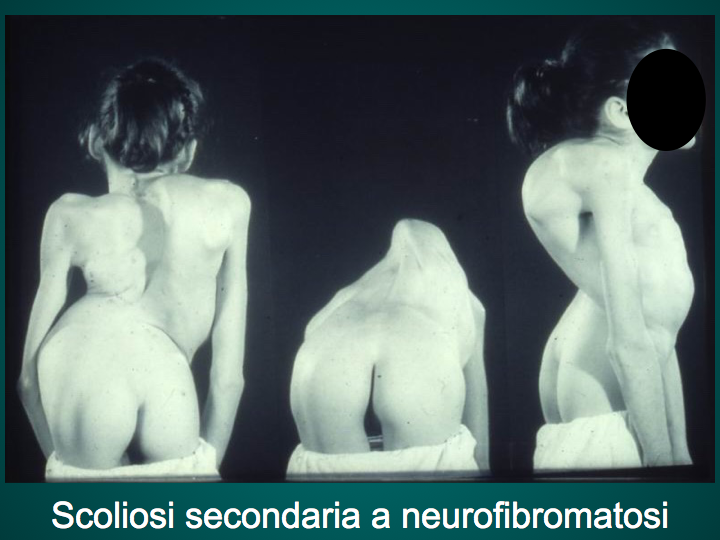
\includegraphics[width=1.62361in,height=3.11667in]{media/image12.png}Pensiamo
al ginocchio come a tre articolazioni:

Femoro-tibiale mediale,

Femoro-tibiale laterale (ognuna con un condilo ,un piatto tibiale e il
menisco ),

Femoro- rotulea

\begin{itemize}
\item
  \textbf{Stress in valgo ed extrarotazione} (ginocchio a x)
\end{itemize}

\begin{quote}
La lesione più frequente, tipico trauma da inforcata degli sci. Può
strappare il collaterale mediale \textbf{LCM}, il \textbf{menisco} tende
a essere schiacciato. Se la forza prosegue anche in senso anteriore si
strappa anche il crociato anteriore \textbf{LCA} e si realizza la
cosiddetta \textbf{``triade sfortunata''}.

Se la forza è davvero eccezionale può sfondare il piatto tibiale. Ci
possono anche essere lesioni associate ai muscoli e del fascio
vascolo-nervoso
\end{quote}

Abbiamo vari \textbf{tipi di distorsione}: distorsione in rotazione
interna ( esempio. giocando a basket), distorsione in rotazione esterna
( esempio. sciando ).

\begin{itemize}
\item
  \emph{\textbf{Trauma in varismo ed intrarotazione}: interessa il
  \textbf{legamento collaterale laterale} (LCL), il \textbf{menisco
  laterale} ed il \textbf{legamento crociato anteriore} (LCA). Se il
  trauma è molto efficiente può interessare anche le strutture del
  compartimento posteriore e le strutture vascolari. }
\item
  \emph{\textbf{Trauma in iperestensione}: può capitare ai calciatori
  quando saltano di testa e atterrano male nella discesa, oppure per
  eventi traumatici diretti. Di solito comporta una lesione del
  \textbf{crociato anteriore} (LCA) e successivamente di quello
  \textbf{posteriore} (LCP). Anche in questo caso, se il trauma è di una
  certa entità possono esserci lesioni del fascio vascolo-nervoso. }
\item
  \emph{\textbf{Trauma diretto}: viene chiamato anche "trauma da
  cruscotto" perché tipico degli incidenti frontali in macchina. Si
  caratterizza come un trauma diretto sulla faccia anteriore della tibia
  a ginocchio flesso (90°). }
\end{itemize}

\emph{Esame clinico}

\begin{itemize}
\item
  È molto importante il \textbf{racconto} \textbf{anamnestico} riguardo
  le modalità traumatiche, improvviso dolore, sensazione di ``crack''
\item
  \textbf{Atteggiamento in semiflessione} con impossibilità alla
  completa estensione →tipica dei menischi
\item
  \textbf{Impotenza funzionale}→ il paziente non può appoggiarsi sul
  ginocchio perché questo cede; sensazione di instabilità.
\item
  \textbf{Tumefazione} ed eventuale presenza di \textbf{versamento
  intra-articolare} con ballottamento rotuleo→ se il ginocchio si è
  gonfiato immediatamente, il versamento è sangue (emartro), se tardivo
  (24-36h) è idrartro.
\end{itemize}

Se all'artrocentesi sono presenti delle \emph{goccioline di grasso},
abbiamo anche una \textbf{frattura.}

\begin{itemize}
\item
  \textbf{Dolore diffuso}, più o meno accentuato e localizzato
\item
  \textbf{Instabilità articolare }
\end{itemize}

Il test più affidabile (100\%) è il \textbf{Lachman test}: l'esaminatore
afferra la tibia e la porta in avanti rispetto al femore. La tibia è
impossibile che si muova se il crociato anteriore è sano (nelle femmine
bisogna valutare le due ginocchia perché queste hanno una lassità
costituzionale maggiore; può essere che la tibia si sposta un po' ma se
ciò accade bilateralmente è normale)

\emph{Esami strumentali}

\begin{itemize}
\item
  \textbf{Radiografia} in proiezioni ortogonali → indispensabile per
  escludere fratture
\item
  \textbf{RMN}→ esame fondamentale insieme alla rx; dà immagini molto
  precise su muscoli, legamenti e menischi
\item
  \textbf{TAC}→ studia bene le ossa ma dà poche informazioni sulle altre
  strutture, può evidenziare fratture non visibili dalla lastra.
\item
  \textbf{Ecografia} →esame secondario; poco informativa su menischi e
  legamenti
\item
  \textbf{Valutazione artroscopica} → si utilizzava anche nella
  diagnostica e per la pianificazione dell'intervento, oggi non viene
  quasi più utilizzata (soppiantata totalmente dalla RMN). Con
  l'artroscopio (dotato di telecamera) si entra all'interno del
  ginocchio disteso da acqua e si possono effettuare varie procedure
  endoscopiche (mediante strumenti adeguati si può tagliare, fresare,
  pulire) di microchirurgia non invasiva.
\end{itemize}

\begin{quote}
\emph{Rottura Meniscale, sintomi e terapia}
\end{quote}

\begin{enumerate}
\def\labelenumi{\arabic{enumi}.}
\item
  Vivo \textbf{dolore}, evidenziare punti di repere di dolorabilità
\item
  \textbf{Versamento} →può essere emartro se viene coinvolta la porzione
  vicino alla capsula oppure un essudato infiammatorio (il gonfiore in
  questo caso si verifica dopo qualche ora e non nell'immediato).
\item
  \textbf{Difficoltà a caricare} o \textbf{blocco articolare} →
  difficoltà ad appoggiare, difficoltà ad estendere e a flettere
\end{enumerate}

La pressione sulla porzione interna o esterna del ginocchio in
corrispondenza del menisco risulterà dolorosa.

L'iperestensione (che schiaccia il menisco) risulterà dolorosa.

La torsione interna-esterna del ginocchio con il paziente a pancia in
giù risulterà dolorosa-

L'artrocentesi metterà in evidenza un liquido che potrà essere limpido o
giallino o emartro.

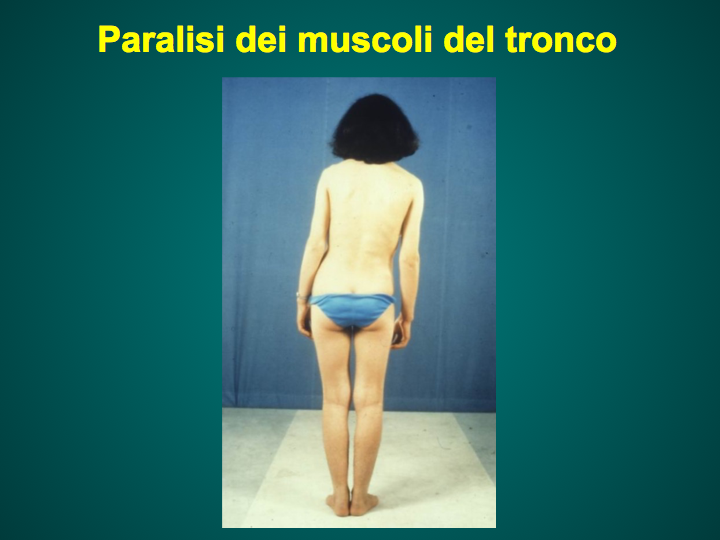
\includegraphics[width=5.33333in,height=2.69792in]{media/image13.png}

\emph{Le \textbf{lesioni meniscali} possono essere isolate o associate a
lesioni capsulo-legamentose e suddivise in:}

\begin{itemize}
\item
  \emph{Lesioni \textbf{traumatiche}: che avvengono durante il
  meccanismo distorsivo, in cui il menisco mediale o laterale si rompe.}
\item
  \emph{Lesioni \textbf{degenerative}: nell'anziano il menisco può
  essere rovinato a causa di lesioni degenerative legate all'usura.}
\end{itemize}

Un menisco si può rompere in diversi modi: dalla semplice fissurazione
alla \textbf{rottura a ``manico di secchio''}. In quest'ultimo caso il
condilo femorale rimane bloccato nel menisco rotto e di conseguenza il
ginocchio rimane bloccato e non può più estendersi (blocco meniscale).

\textbf{Test di Apley}

Si mette il paziente prono (a pancia in giù), si piega il ginocchio a
90°, si prende la pianta del piede, si schiaccia contro il lettino e si
fanno dei movimenti di intra/extrarotazione del piede. Questo determina
una compressione del femore sulla tibia, cui consegue uno schiacciamento
dei menischi che, se rotti, fanno male.

Se extraruoti il piede hai di solito un dolore mediale, sinonimo di una
lesione del menisco mediale; viceversa, se intraruoti il piede hai un
dolore laterale, sinonimo di una lesione del menisco laterale.

\textbf{TERAPIA}

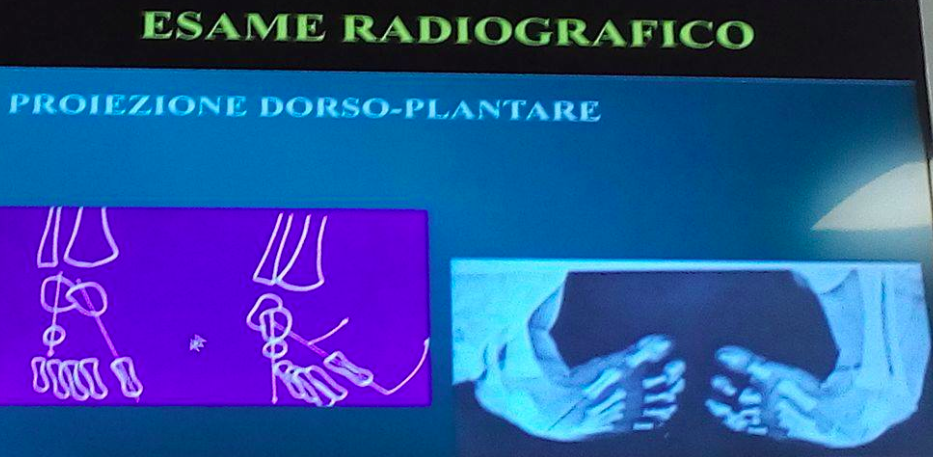
\includegraphics[width=2.34167in,height=2.58056in]{media/image14.png}Il
menisco ha una crepa, con strumenti adeguati (bisturi taglienti) si
recide la parte danneggiata (in passato si toglieva tutto il menisco,
oggi si toglie il meno possibile).

Un menisco degenerato è più facile che si rompa anche con un trauma
modesto. Ci sono vari gradi di rottura meniscale. Quando il menisco è
rotto in corrispondenza della capsula in modo lineare può essere anche
suturato (questi sono casi molto selezionati). Soltanto la porzione di
menisco attaccata alla capsula è vascolarizzata (è impensabile che
qualcosa cicatrizzi in una zona priva di vascolarizzazione) e una
lesione a questo livello sanguina (emartro) .

Trapianti meniscali da cadavere → eccezionalmente (pochissimi casi
all'anno in Emilia Romagna) si possono fare trapianti meniscale da
cadavere. Riguardano solo pazienti giovani in cui tutto è sano e solo il
menisco è irrecuperabile

\emph{Lesioni di legamenti collaterali }

\begin{itemize}
\item
  Vivo dolore → dolore sulla emirima, sulla inserzione femorale e
  tibiale
\item
  Scarso o assente versamento ematico
\item
  Instabilità del ginocchio
\end{itemize}

\textbf{Test in valgismo o abduzione }

Valuta l'integrità del \textbf{legamento collaterale mediale} (LCM).
Valgizzo il ginocchio a ginocchio esteso e flesso. Se ho una lesione del
LCM, il ginocchio di aprirà di più rispetto al controlaterale.

\textbf{Test in varismo o adduzione }

Valuta l'integrità del \textbf{legamento collaterale laterale} (LCL). Se
vi è una lesione, il ginocchio si aprirà di più lateralmente rispetto al
controlaterale.

Questi due test (Fig. 54) vengono fatti con il ginocchio flesso di circa
20°-30° e bisogna sempre confrontare con il ginocchio controlaterale.

\textbf{GRADI DI DANNO} :

\begin{itemize}
\item
  \textbf{Primo grado} → stressare la lesione provoca molto dolore (è
  come se andassimo a schiacciare su un livido, fa male)
\item
  \textbf{Secondo grado} → fa molto male (il collaterale è parzialmente
  integro)
\item
  \textbf{Terzo grado} → il collaterale è tutto strappato →
  paradossalmente non fa male e il ginocchio è instabile
\end{itemize}

\emph{Lesione legamento crociato anteriore }

Il crociato anteriore si inserisce su spina tibiale e gola.

Meccanismi lesionali su questa slide (lui ha detto sul libro)

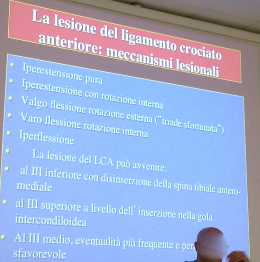
\includegraphics[width=3.85417in,height=3.73958in]{media/image15.png}

Sintomi di rottura LCA

\begin{itemize}
\item
  Dolore più o meno intenso (non eccessivo)
\item
  Versamento ematico (non sempre)
\item
  Instabilità
\end{itemize}

\textbf{Manovra di Lachman: }

\begin{enumerate}
\def\labelenumi{\arabic{enumi}.}
\item
  \textbf{Cassetto anteriore} →il paziente deve essere rilassato
  (difficile i primi giorni perché il ginocchio fa male) e l'esaminatore
  porta la tibia in avanti come se aprisse un cassetto (nel mentre tiene
  fermo il piede per stabilizzarlo): se è rotto il crociato anteriore la
  tibia scivola in avanti, tanto più se viene extraruotato un po' il
  piede.
\item
  \textbf{Cassetto posteriore} → se è rotto il crociato posteriore la
  tibia scivola indietro anche per semplice gravità (tenendo in alto il
  piede si forma un avvallamento in corrispondenza del ginocchio cioè
  scende la tuberosità). Naturalmente si fa sempre il paragone con il
  controlaterale.
\end{enumerate}

\begin{quote}
La lesione del LCA può essere fresca (ci sono ancora tutti i vasi
strappati) o spenta (conica).

In pazienti con lesioni reiterate la contrazione del quadricipite può
determinare un ``auto cassetto''

\emph{Terapia per la rottura LCA}

È \textbf{solo chirurgica} e non si fa in urgenza, cioè si aspetta che
l'infiammazione si risolva. Non si può suturare un tendine ma lo si deve
\emph{sostituire}. Principalmente si usano due sostituti che derivano
da: tendine rotuleo, gracile e semitendinoso, tendine di donatore,
legamento artificiale.

Nei giovani si preferisce utilizzare il tendine rotuleo, gracile e
semitendinoso; negli anziani o se c'è la necessità di recuperare molto
in fretta si utilizza un legamento artificiale\textbf{. }

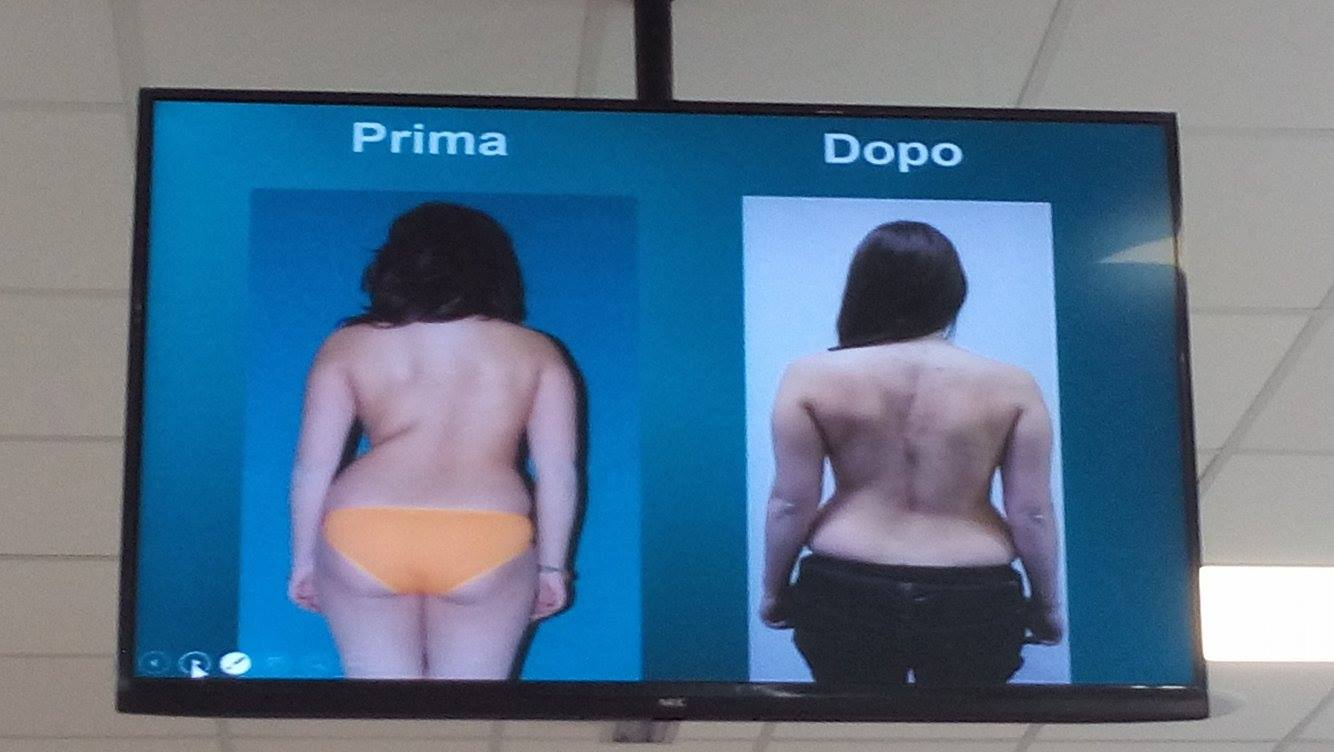
\includegraphics[width=2.42847in,height=2.24861in]{media/image16.jpeg}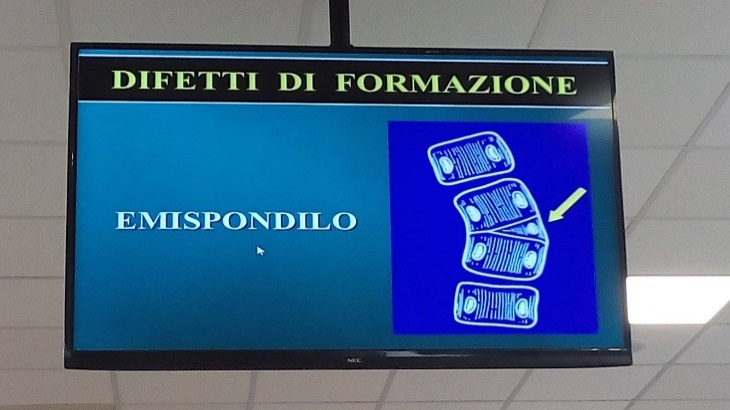
\includegraphics[width=3.20833in,height=2.26042in]{media/image17.jpeg}

\textbf{Ricostruzione con tendine rotuleo}: si usa la parte centrale del
tendine con 2 porzioni ossee alle estremità; si fa un tunnel dalla tibia
al femore e si fa passare il nuovo legamento (attraverso 2 fili legati
alle estremità), le due porzioni ossee andranno a chiudere il tunnel
osseo e si salderanno mentre la parte tendinea rimarrà intrarticolare.

\textbf{Ricostruzione con tendine gracile e semitendinoso}: sono
utilizzati insieme , vengono tubulizzati, misurati ( si fanno dei
calcoli anche della dimensione del tunnel); vengono fissati a livello
dei tunnel ossei mediante viti a interferenza che schiacciano l'osso
contro la parete del nuovo legamento.

\textbf{LESIONI CARTILAGINEE}→ raramente acute; più frequentemente sono
il risultato di \textbf{usura cronica}; nessuno al mondo ha risolto il
problema della ricostruzione cartilaginea ( altrimenti avremmo vinto
l'artrosi). Si possono ricostruire piccole parti di cartilagine ma non
sarà mai cartilagine ialina.

Esempio di lesione cartilaginea in acuto: un pezzo di cartilagine + osso
subcondrale si è staccato dal condilo, in questo caso si può intervenire
perché è una lesione fresca e si può riattaccare osso con osso. Lo si
fissa con chiodini biodegradabili e con delle micro viti. Questo è un
caso molto fortunato.

Quando invece la cartilagine ha dei danni inveterati si fanno delle
\textbf{microperforazioni} in modo da far salire del sangue dall'osso
subcondrale e con questo anche le cellule staminali, poi si comprime con
una membrana di collagene sperando che si formi almeno della
fibrocartilagine.

La seconda alternativa consiste negli \textbf{innesti di cartilagine}.
Tecnica mai tramontata è quella di mettere dei piccoli cilindri di
cartilagine che vengono prelevati da altre sedi.

Altra tecnica consiste nel posizionare dei grossi cilindri che si
adattano benissimo (grossa limitazione: bisogna danneggiare un'altra
parte del ginocchio per poter ottenere questi cilindri).

Oggi ci si affida soprattutto al \emph{trapianto di cartilagine}, quindi
al prelievo di cartilagine, alla sua espansione, all'ottenimento dei
\emph{condrociti autologhi} che vengono \emph{coltivati} dentro delle
membrane di acido ialuronico che infine vengono posizionate.

Limitazioni → doppio intervento, aree di limitate dimensioni, costi
elevati. Comunque sia non si otterrà mai quel punto di passaggio fisso
tra cartilagine e osso; ci sarà sempre un certo effetto onda che
difficilmente farà durare la cartilagine negli anni.

Qualsiasi sia la tecnica, è sempre fallimentare se non si interviene
sulla \textbf{causa primaria} (varismo, lesione LCA\ldots{}). Di fronte
ad un \emph{\textbf{ginocchio varo}} dove il carico e l'usura è tutta
sul condilo mediale non sarà possibile fare cartilagine se non prima di
aver raddrizzato chirurgicamente le ginocchia (\emph{osteotomia
valgizzante}→ sezione a cuneo della tibia, raddrizzamento e
posizionamento di una placca).
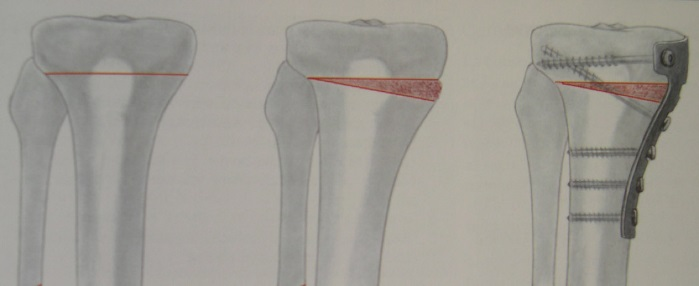
\includegraphics[width=3.17708in,height=1.30208in]{media/image18.jpeg}

Artroscopia

Entriamo attraverso piccoli fori all' interno dell'articolazione che
viene distesa da liquido ( la pancia da gas) ai fini di ispezione
(soppiantata da RMN) oppure si può utilizzare strumenti manuali o
motorizzati per correggere il difetto.

Un menisco normale lo si vede tra femore e tibia ed è sano, lucente in
un giovane; sarà triangolare e cioè largo alla base e assottigliato
verso il centro. Il menisco esterno è più chiuso e talvolta discoide.

Il legamento crociato anteriore normale è bianco e teso. Il crociato
posteriore si vede sempre male. Le cartilagini normali sono lisce e
lucenti. La gola femoro-rotulea normale si vede con la tipica concavità
e convessità. L' articolazione femoro-rotulea normale è caratterizzata
da cartilagine teso-elastica che non si lascia sfaldare.

ANATOMIA ARTROSCOPICA PATOLOGICA → carrellata di immagini artroscopiche
(non riportate tutte) su:
\end{quote}

\begin{itemize}
\item
  Menisco degenerato di paziente anziano \textbf{1}
\item
  Menisco esterno discoide → menisco a ``o'', tutto fuso
\item
  Rottura meniscale con danno cartilagineo
\item
  Lesione ``a manico di secchia'' → il condilo si va ad infilare tra i
  due elementi meniscali rotti \textbf{2}
\item
  Lesione menisco mediale
\item
  Flap meniscale →Menisco rotto ripiegato su se stesso
\item
  Menisco degenerato e rotto su un quadro di tipo artrosico senile
\item
  Articolazione femoro-rotulea patologica → rotula sfrangiata per una
  sofferenza cartilaginea
\item
  Sinoviti in artrite reumatoide → la membrana sinoviale diventa
  villosa, basta toccarla e sanguina (anche nelle forme psoriasiche)
\item
  Crociato anteriore rotto →anche la guaina non c'è più
\item
  Lesione completa subacuta del crociato anteriore → con tutti i suoi
  vasi
\item
  Lesione completa cronica del crociato anteriore
\end{itemize}

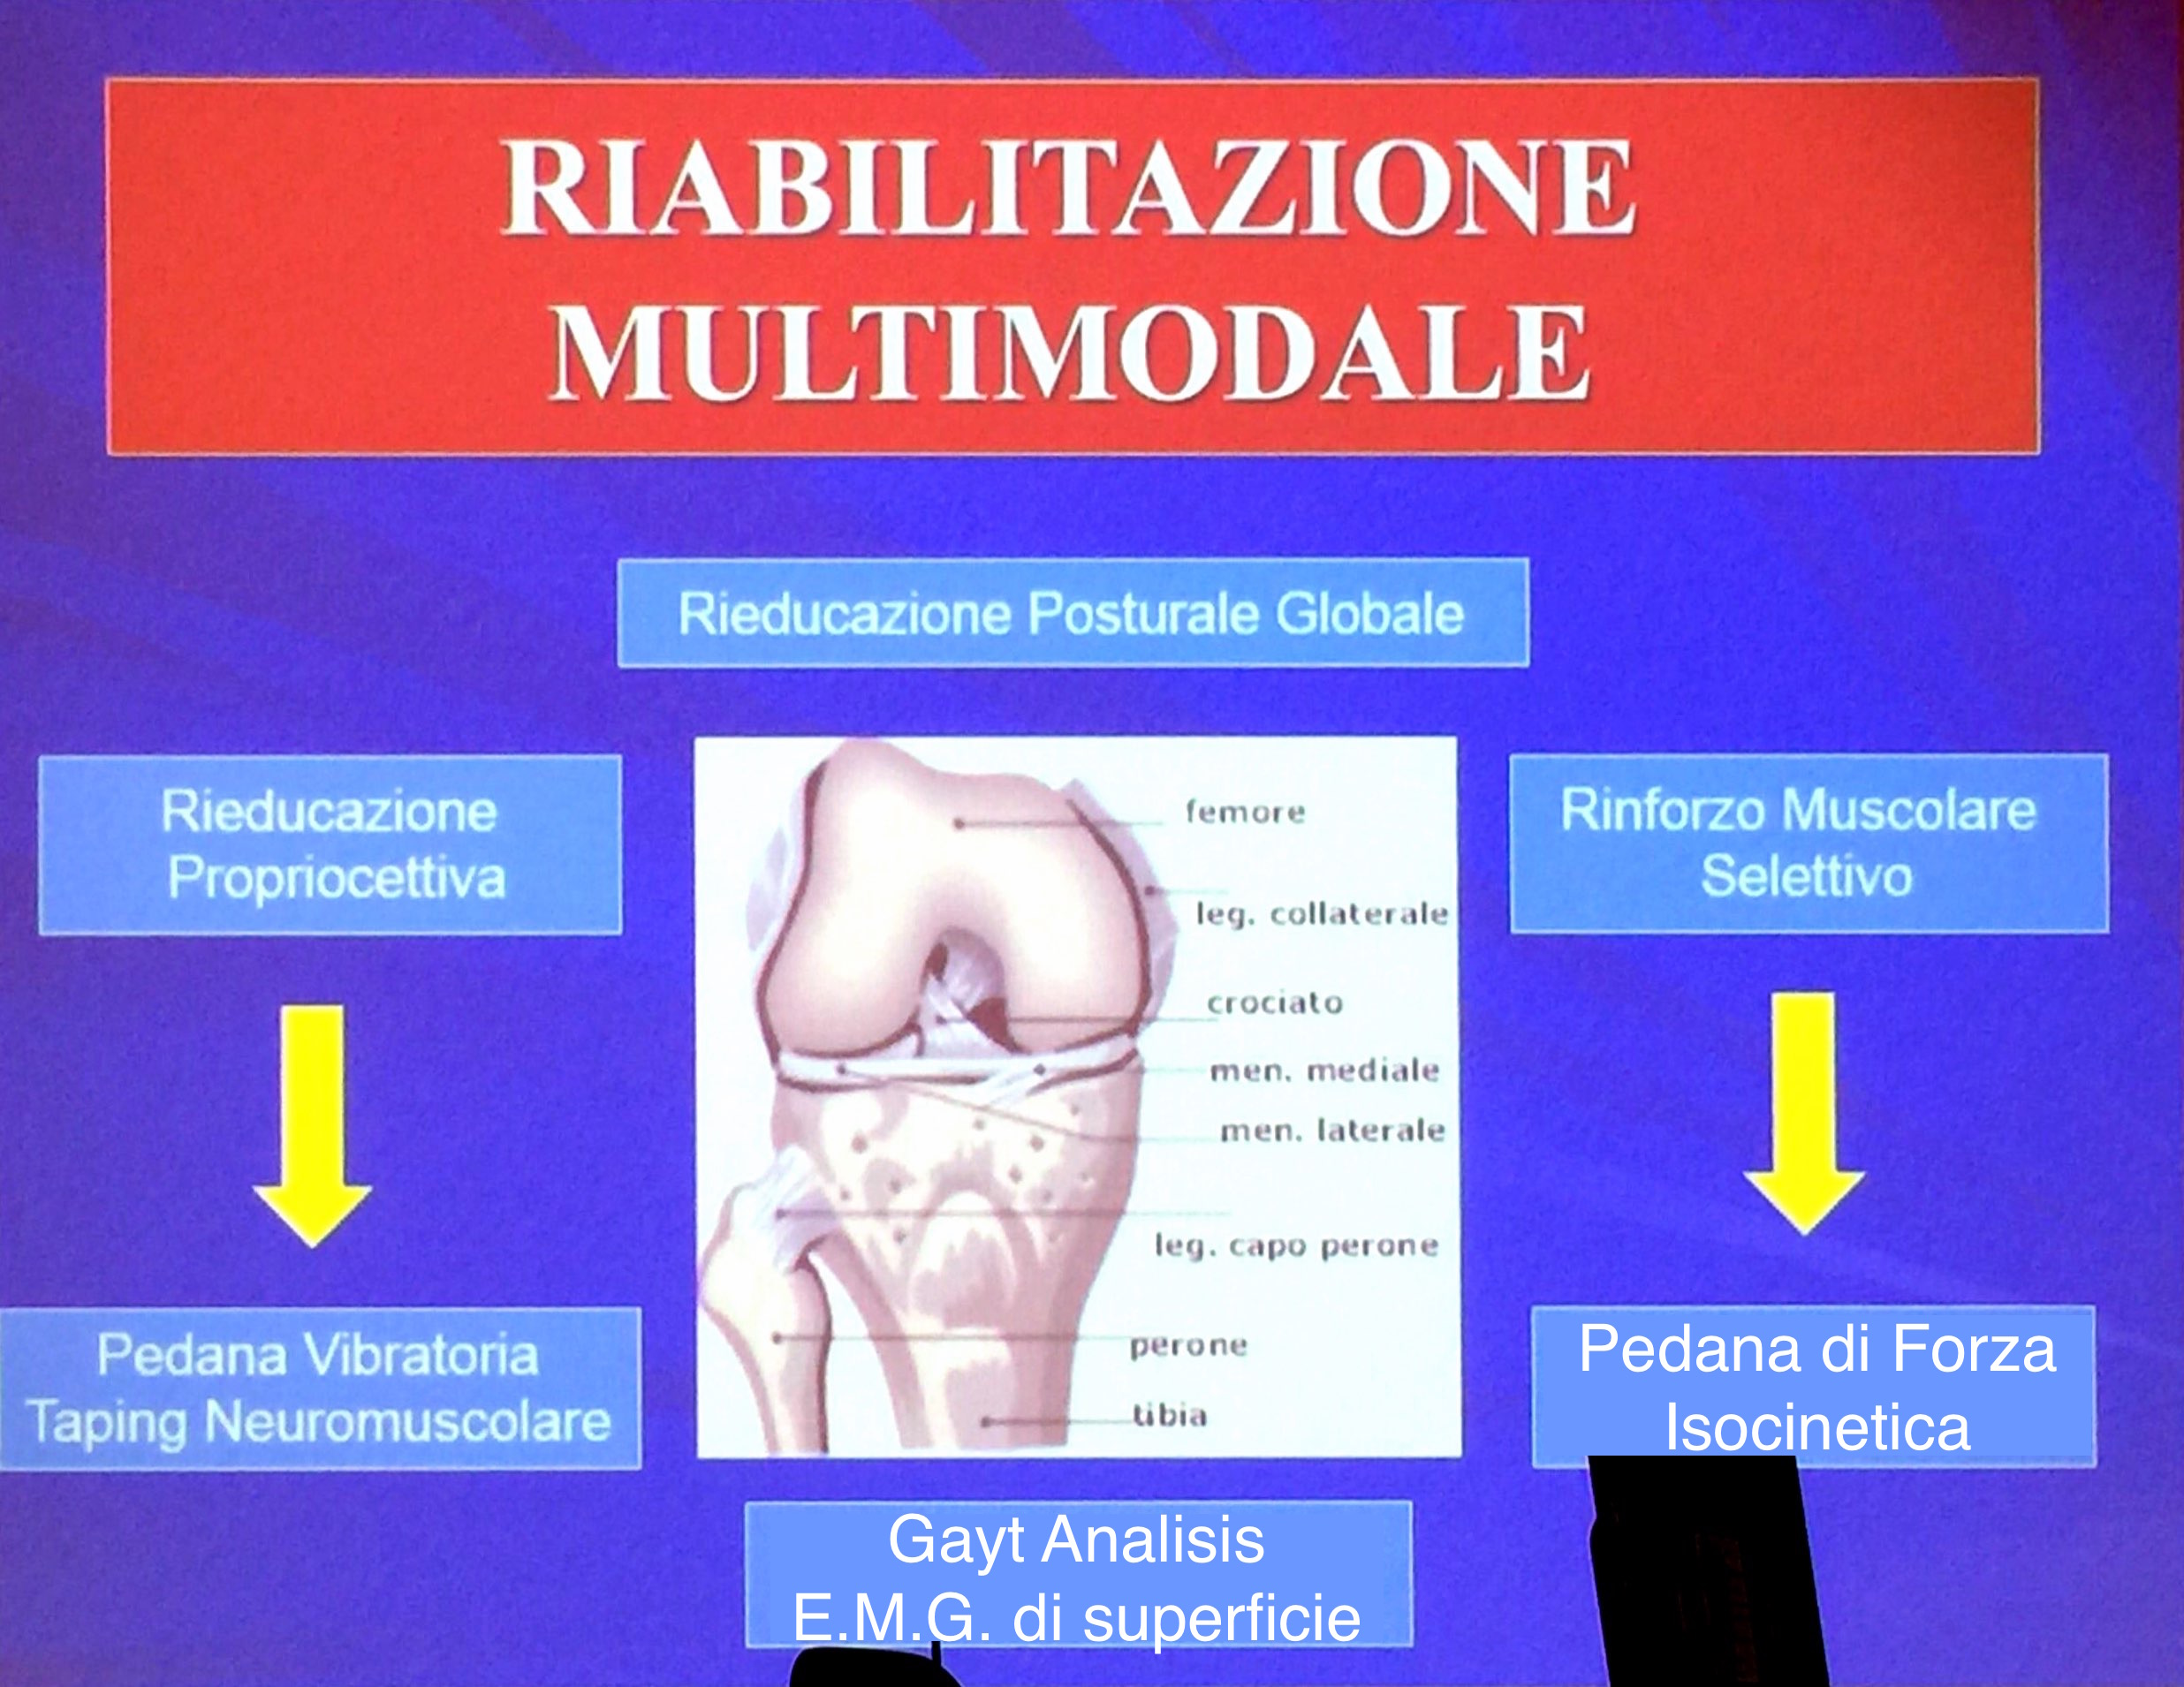
\includegraphics[width=3.05208in,height=2.44792in]{media/image19.jpeg}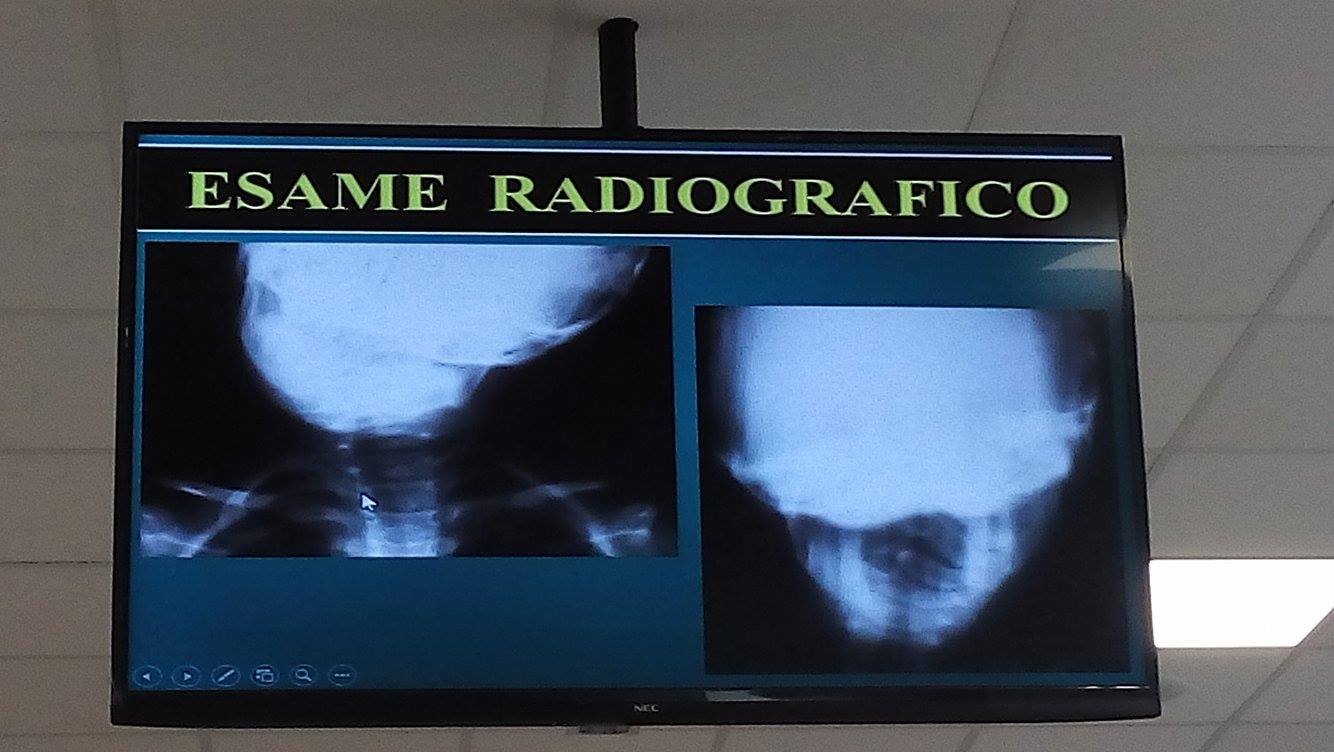
\includegraphics[width=3.09375in,height=2.46875in]{media/image20.jpeg}

PATOLOGIA DEGENERATIVA DEL GINOCCHIO

È \textbf{l'artrosi del ginocchio o gonartrosi}.

Colpisce i versanti articolari femoro-tibiale (mediale e laterale ;
entrambe o isolatamente) e femoro-rotuleo (isolatamente o in
associazione ai compartimenti femoro-tibiali).

Può essere primitiva o secondaria. Nella \emph{primitiva} non si
individua una causa all'origine e colpisce l'età avanzata. Le ginocchia
per tutta la vita subiscono (non essendo delle sfere le SUBISCONO) delle
sollecitazioni notevoli soprattutto rotatorie tanto più se poi c'è
artrosi d'anca ed elevato peso corporeo (esiste il ``ginocchio
dell'obeso'') → artrosi senile .

Nell' artrosi \emph{secondaria} si conosce la causa e può comparire
anche in età giovane a seguito di una frattura complessa del piatto
tibiale, deviazioni assiali costituzionali femoro-tibiali, disassamenti
femoro-rotulei (la rotula devia), trauma (fratture complesse
irrecuperabili o fratture non perfettamente aggiustate dal chirurgo),
dismetria, artrite, lesioni meniscali , obesità.

\emph{Clinica }

\begin{itemize}
\item
  Tumefazione → da infiammazione o da deformità ossee
\item
  Deformità
\item
  Dolore → ``di fuga''
\item
  Rigidità → il ginocchio rimane semiflesso
\item
  Zoppia → zoppia di fuga o zoppia da ipometria relativa
\item
  Sovraccarichi → il ginocchio che lavora male potrà infiammare l'altro
  ginocchio, l'anca o la schiena
\end{itemize}

\begin{quote}
Ginocchio atrosico varo e campo chirurgico

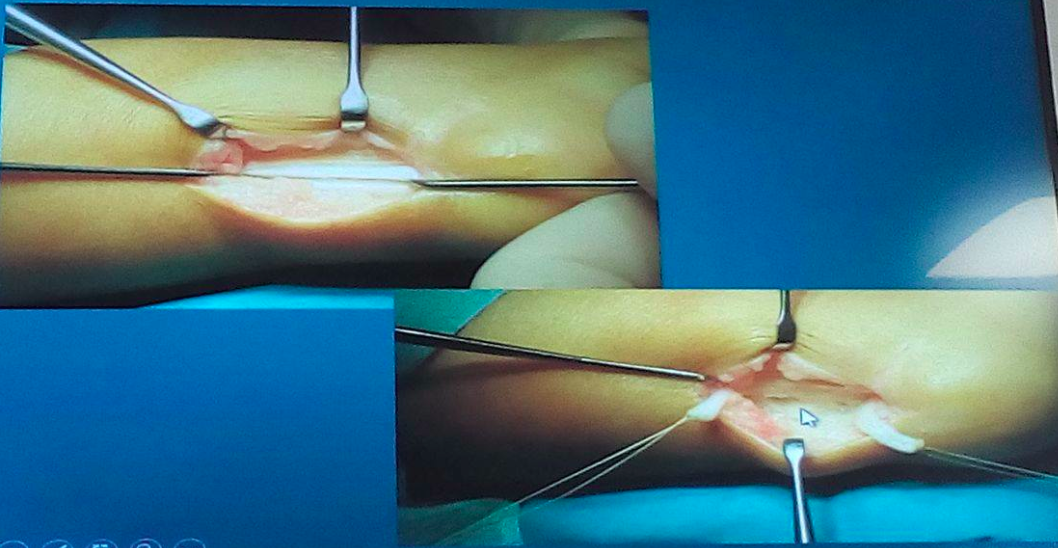
\includegraphics[width=3.93750in,height=2.29167in]{media/image21.png}

Artrocentesi → Idrarto (liquido sieroso, citrino , limpido) -- Emartro
(emofilico o post-traumatico) -- Versamento purulento (infezione),
artrite suppurativa.

NB: versamento giallo, citrino, torbido → potrebbe essere Gotta

Il ginocchio non presenta più le sue naturali pieghe e incavi ma si
presenta ``Balliforme'' poiché è pieno di liquido. Segno del
ballottamento rotuleo → Schiacciando avrete la possibilità di abbassare
la rotula come un galleggiante nell'acqua ( dopo la compressione la
rotula risale perché il liquido recupera la sua sede ). Tramite
l'artrocentesi , fatta in uno spazio compreso tra rotula e condilo
femorale, si fa evacuare questo liquido.

\emph{Esami strumentali }

Radiografia :
\end{quote}

\begin{itemize}
\item
  \textbf{Riduzione o scomparsa} della \textbf{rima articolare}, cioè
  dello spazio normalmente trasparente che divide i 2 capi articolari (
  es. ginocchio varo in cui c'è una scomparsa della rima solo nella
  parte mediale)
\item
  \textbf{Deformazione capi articolari} → non essendoci più la
  cartilagine, l'osso subcondrale si rimodella (es. paziente con artrite
  reumatoide, sinovite aggressiva, erosione dei capi articolari e
  artrosi diffusa che coinvolge tutte le cartilagini.
\item
  \textbf{Osteoporosi} e addensamenti
\item
  Geodi, osteofiti
\end{itemize}

\emph{Terapia }

\textbf{TERAPIA MEDICA }

\begin{enumerate}
\def\labelenumi{\arabic{enumi}.}
\item
  Ridurre i carichi (se il paziente è in sovrappeso deve dimagrire, non
  fare sforzi)
\item
  Mantenere l'escursione articolare e muscolare (ginnastica)
\item
  Fisioterapia (ultrasuoni, laser)
\item
  Terapia farmacologica (antiinfiammatori, antidolorifici,
  condroprotettori per os, infiltrazioni intra-articolari di acido
  ialuronico)
\end{enumerate}

\textbf{TERAPIA CHIRURGICA }

\begin{itemize}
\item
  Conservativa nei casi meno gravi (es. un ginocchio vago-valgo può
  essere raddrizzato ridistribuendo i carichi)
\item
  Protesica mono-compartimentale nei casi più gravi
\item
  Delle complicanze
\end{itemize}

Medializzazione del carico → paziente di 42 anni con ginocchio varo (il
carico è sulla porzione mediale). La cartilagine è tutta ``pelosa'' e
sciupata, la rima è scomparsa a livello mediale ; il chirurgo attua un'
interruzione e allarga di un tot di gradi, spostando il carico
maggiormente sul lato sano.

Ginocchio valgo artrosico → generalmente il problema è femorale e si
interviene con più difficoltà con una osteotomia femorale . NB: se il
\emph{bambino} ha le ginocchia molto storte conviene intervenire subito
in quanto basta bloccare la crescita da un lato con delle graffettine
epifisarie asimmetriche transitorie; senza fare nient'altro un ginocchio
valgo si raddrizzerà da solo.

\textbf{SOSTITUZIONE PROTESICA }

Se tecniche artroscopiche, osteotomie ecc. non sono sufficienti o se
comunque il danno è molto importante si interviene con la sostituzione
protesica. Può essere:

\begin{itemize}
\item
  Mono-compartimentale (solo la femoro-tibiale)
\item
  Bi-compartimentale (o le 2 femoro-tibiali o una femoro-tibiale insieme
  ad una femoro-rotulea),
\item
  Tri-compartimentale (tutte).
\item
  Bimonocompartimentale significa sostituzione protesica
  monocompartimentale in entrambe le ginocchia.
\item
  Bitricompartimentale → sostituzione tricompartimentale in entrambe le
  ginocchia
\item
  Protesi post-traumatica → molto difficile , si attua con protesi
  particolari adatte alla anatomia alterata
\end{itemize}

\begin{quote}
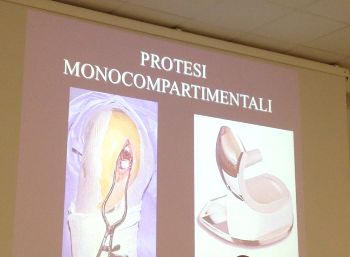
\includegraphics[width=3.05208in,height=2.23958in]{media/image22.png}
\end{quote}

La protesi rotulea è di solo polietilene , di sola plastica e quindi con
la radiografia non si può vedere. La sostituzione protesica non serve
per raddrizzare le gambe storte ,infatti ci sono dei limiti : se le
gambe sono troppo storte non si può fare la sostituzione in quanto la
protesi viene sollecitata e sparata fuori.

\emph{Complicanze }

\begin{itemize}
\item
  Infezioni (nella rx si vede del nero intorno alla protesi) → bisogna
  togliere la protesi e mettere una falsa protesi di cemento caricata di
  antibiotici (per 2-3-4 mesi); somministriamo antibiotici e quando
  abbiamo estirpato l'infezione sostituiamo con la vera protesi.
\item
  Mobilizzazione asettica.
\item
  Frattura periprotesica.
\end{itemize}

Risposte a dubbi sulla patologia del ginocchio :

\begin{itemize}
\item
  Non esiste la possibilità di fare iniezioni di cartilagine, possiamo
  fare solo iniezioni di acido ialuronico ( a minore peso molecolare nei
  giovani per nutrire la cartilagine , a più alto peso molecolare per
  lubrificare negli anziani )
\item
  I trapianti di cartilagine esistono ma si fanno solo in pazienti
  giovani, motivati e in zone molto limitate. Non siamo in grado di
  ricostruire il tessuto ingegnerizzato e cioè cartilagine ialina,
  tessuto subcondrale, osso spongioso
\item
  Le cellule staminali possono avere un ruolo ma molto limitato
\end{itemize}

\end{document}
